\documentclass[../jb_user_manual.tex]{subfiles}
\begin{document}


\subsection{\Large{How to Use}} 

The JuiceBox is intended to serve as a battery powered AC supply and includes an integrated battery charger.  120 VAC output in the form of a standard wall outlet is available on the casing, while the charger input takes the form of a standard extension cable.  Device performance information is displayed on an integrated display (shown below).

\vspace{3mm}
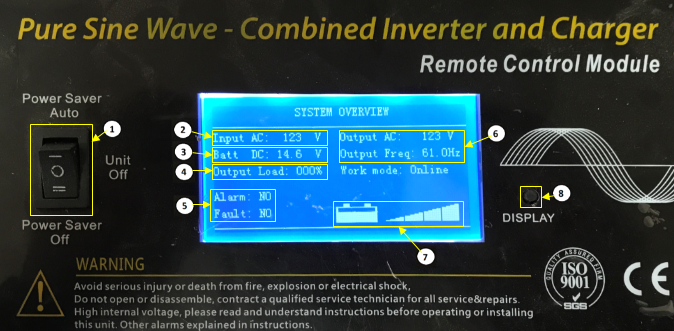
\includegraphics[width=6in]{display_3}
\vspace{3mm}

\begin{enumerate}
	\item{Dual-Mode Power Switch}
	\item{Charger Input Voltage}
	\item{Battery Pack DC Voltage}
	\item{Output Load (Percentage of 2000W Capacity)}
	\item{Alarm/Fault Indicator}
	\item{Output Voltage and Frequency}
	\item{Battery Charge Indicator}
	\item{Display Wakeup Button}
\end{enumerate}

The JuiceBox power switch has three settings, "Power Saver Off", "Power Saver Auto", and "Unit Off". ************DESCRIBE*********  The battery charge indicator displays the battery charge level in 25 percent increments, with all four sections illuminated when the device is above 75 percent charge.  The display wakeup button is used to wake the display from sleep mode when the device is powered on.  The alarm indicator registers a low battery alarm, while the fault indicator monitors the occurrence of over-current faults in which the load exceeds device capacity.  Exceeding device current limits will trip the internal breaker; to reset this breaker, fully depress the corresponding button located on the device casing (shown below).

\vspace{3mm}

\includegraphics[width=6in]{ssi_logo}
\vspace{3mm}

\subsection{\Large{Charging the JuiceBox}}

The juice box should be charged for a minimum of 8 hours following full discharge to restore to full charge.  Draining the batteries frequently and failing to fully recharge them in between uses may degrade the batteries, resulting in reduced battery life.  The device can be charged by plugging the charging cord into any standard 120 VAC wall outlet and turning the power switch to one of the "on" settings. If the unit is not set to "On", the batteries will not recharge.*****IS THIS TRUE?*****

\subsection{\Large{Battery Life}}

The juice box can supply up to 16.5 A at 120 VAC.  Battery life is related to current draw; for greater loads, corresponding battery life is reduced.  The graph below shows the relationship between maximum battery life and the percentage of the maximum load.

\vspace{3mm}
\includegraphics[width=6in]{battery_life}
\vspace{3mm}

\hangindent = 1.8cm
\hangafter = 1
Note: Graph depicts maximum battery life for new unit with fresh batteries at full charge.  Low power alarm will sound before reaching full discharge.

\end{document}